% Metódy inžinierskej práce

\documentclass[10pt,twoside,english,a4paper]{article}

\usepackage[english]{babel}
%\usepackage[T1]{fontenc}
\usepackage[IL2]{fontenc} % lepšia sadzba písmena Ľ než v T1
\usepackage[utf8]{inputenc}
\usepackage{graphicx}
\usepackage{url} % príkaz \url na formátovanie URL
\usepackage{hyperref} % odkazy v texte budú aktívne (pri niektorých triedach dokumentov spôsobuje posun textu)

\usepackage{cite}
%\usepackage{times}

\pagestyle{headings}

\title{Benefits of Implementing Gamification in Health \& Wellbeing and the Ethics behind It\thanks{Semester project in the subject Methods of engineering work, ac. year 2022/23, leaading: Fedor Lehocki}} % meno a priezvisko vyučujúceho na cvičeniach

\author{David Truhlar\\[2pt]
	{\small Slovak University of Technology in Bratislava}\\
	{\small Faculty of Informatics and Information Technologies}\\
	{\small \texttt{xtruhlar@stuba.sk}}
	}

\date{\small 05/10/2022} % upravte



\begin{document}

\maketitle

\begin{abstract}
The use of game elements in real-life context for different non-game purposes is increasingly popular today and the gamification of Health and Wellbeing is not an exception. Gamified apps have enormous potential to motivate people to move and exercise regularly, simplify bureaucratic processes, or help educate medical staff in their areas of practice. Yet gamification of healthcare carries potential risks and ethical questions about privacy and misuse of medical records to name just a few. This article will discuss the positive impacts as well as drawback of gamification and provide final conclusions.
\end{abstract}

%
%
%

\section{Introduction}
"Gamification", known as using game elements and techniques  in non-game contexts to motivate and increase user activity \cite{Gamefulness} has become very popular in last decade. These elements are features as levels, rewards, earning points and badges or getting better rank in leader-boards. This topic instantly initiate public debate and every industry ranging across productivity, finance, education, news etc. \cite{Gamefulness} started implementing these ideas in their field. The social networks as Facebook and Instagram and other similar platforms, have contributed to an increase in using of "gamification", in order to improve interaction and engagement with their users. 

Using '"gamified" apps and features ind health became as popular as in other areas, and currently is becoming today's standard. These rewards and badges often aims to encourage health activities and help people to live healthier life-style. The pandemic of Covid-19 also changed the way we are looking on the implementing these principles in the real word in the terms of education and training of the medical stuff.  There are already a few researches on benefits of these principles but there are many risks that have to be covered, to say that "gamification" in health is only beneficial, too. Mostly, these challenges have ethical character which means their elimination should be achievable,  as they are the "human-factor" type of problems.

After the presenting what "gamification" in health means this article will discuss some benefits in the~\ref{benefits} section. In the next part, I will examine risks and possible dangers connected to "gamification" in the~\ref{risks} section. In the end, I will review some solutions for the challenges and summarize my conclusions in the~\ref{summary} section.

%
%
%

\section{"Gamification" in health} \label{G-i-H}
In the context of health and well-being is the main goal of "gamified" elements generally changing user's behavior by increasing their activity and and/or practicing healthier life-style via game-like experience. The main reason why is "gamification" so popular in last years is strongly link with the  accessibility of digital technologies, particularly smart phones as well as digital infrastructure\cite{Ethics} that has been created and have connected the whole world. 

The health trackers and health apps have millions of users today, and the competition in this field is enormous.In The research "Global Healthcare Gamification Market Analysis and Trends - Industry Forecast to 2025" done by Research and Markets the estimated market gap for "gamification" in healthcare will reach 13.58 billion by 2025. \cite{mgap}  One of the most obvious examples of companies that implemented gamified elements successfully in their market strategies is Apple, with ecosystem created between users Apple Watch and iPhone where user is rewarded for accomplishing tasks connected to movement - steps, calories and the count of hours user was active.  Apple also awards people on special days, as Earth Day (April 22.) when user can get 'special' badge for exercising more than 30 minutes that day\cite{earthDay}. All of these apps focus on users activity such steps, kilometers run or the amount of burned calories per day. The motivation begin when user start collecting the badges for completed goals and their position in leader-board is getting better. This can also be applied to mental health or basic daily tasks as reminders to drink enough water, take one's pills or keep track of the sleep routine.

%
%
%

\section{Benefits} \label{benefits}

Základným problémom je teda\ldots{} Najprv sa pozrieme na nejaké vysvetlenie (časť), a potom na ešte nejaké (časť.\footnote{Niekedy môžete potrebovať aj poznámku pod čiarou.}

Môže sa zdať, že problém vlastne nejestvuje, ale bolo dokázané, že to tak nie je. Napriek tomu, aj dnes na webe narazíme na všelijaké pochybné názory. Dôležité veci možno \emph{zdôrazniť kurzívou}.


\subsection{The most used features} \label{benefits:features}

%
%
%

\section{Risks} \label{risks}

%
%
%

\section{Summary} \label{summary} % prípadne iný variant názvu

%
%
%

\section{zvasty zo vzoru}\label{zvasty}
%Z obr.~\ref{f:rozhod} je všetko jasné. 

\begin{figure*}[tbh]
\centering
%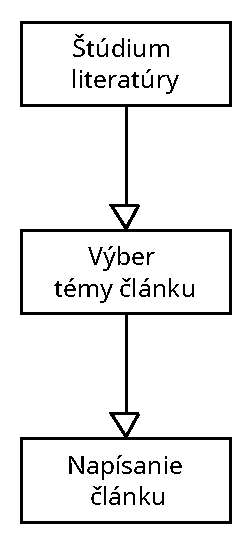
\includegraphics[scale=1.0]{umletino_diagram.pdf}
%Aj text môže byť prezentovaný ako obrázok. Stane sa z neho označný plávajúci objekt. Po vytvorení diagramu zrušte znak \texttt{\%} pred príkazom \verb|\includegraphics| označte tento riadok ako komentár (tiež pomocou znaku \texttt{\%}).
\caption{Rozhodujúci argument.}
\label{f:rozhod}
\end{figure*}


 Niekedy treba uviesť zoznam:

\begin{itemize}
\item jedna vec
\item druhá vec
	\begin{itemize}
	\item x
	\item y
	\end{itemize}
\end{itemize}

Ten istý zoznam, len číslovaný:

\begin{enumerate}
\item jedna vec
\item druhá vec
	\begin{enumerate}
	\item x
	\item y
	\end{enumerate}
\end{enumerate}

%\acknowledgement{Ak niekomu chcete poďakovať\ldots}

\paragraph{Veľmi dôležitá poznámka.}
Niekedy je potrebné nadpisom označiť odsek. Text pokračuje hneď za nadpisom.


% týmto sa generuje zoznam literatúry z obsahu súboru literatura.bib podľa toho, na čo sa v článku odkazujete
\bibliography{lit1}
\bibliographystyle{plain} % prípadne alpha, abbrv alebo hociktorý iný
\end{document}
